
%(BEGIN_QUESTION)
% Copyright 2006, Tony R. Kuphaldt, released under the Creative Commons Attribution License (v 1.0)
% This means you may do almost anything with this work of mine, so long as you give me proper credit

In this continuous cookie-baking process, cookies are transported through an oven on a conveyor, the temperature of the cookies being measured ``downstream'' of the oven.  A non-contact temperature transmitter is used in this process for sanitary reasons, so that the instrument never physically contacts the food:

$$\includegraphics[width=15.5cm]{i00110x01.eps}$$

Suppose that the transport time of the cookies from the oven to the point where the infra-red pyrometer senses their temperature is 15 seconds.  In process control terms, what is this delay called, and what effect will it have on the stability of control in this system?

\vskip 20pt \vbox{\hrule \hbox{\strut \vrule{} {\bf Suggestions for Socratic discussion} \vrule} \hrule}

\begin{itemize}
\item{} Explain how you might improve the performance of this control system. 
\item{} Explain how the temperature transmitter (TT) senses cookie temperature.  Specifically, what physical principle(s) does this transmitter use to perform its measurement?
\end{itemize}

\underbar{file i00110}
%(END_QUESTION)





%(BEGIN_ANSWER)

This delay is commonly referred to as {\it dead time} (or {\it transport delay}), and it wreaks havoc with feedback control systems because the controller only sees the delayed results of its control action.  This is analogous to driving an automobile by looking {\it backward} out the rear window, controlling the steering wheel in response to the road you've already driven over!

%(END_ANSWER)





%(BEGIN_NOTES)

The problem in this system is not the time the cookies spend in the oven, but rather the time they spend between emerging from the oven and being sensed by the infra-red temperature transmitter.  This delay is called ``dead time,'' and it is a bad thing in any control system.

Dead time should be eliminated from process control loops wherever possible, just as deadband and hysteresis should be eliminated in process sensing and control instruments (transmitters and valves).  Either type of ``dead'' effect makes the process seem completely unresponsive to the control system's action, at least within a certain range of motion or time.  Since one of the foundational principles of process control is that you cannot control what you do not measure, this means the oven control system cannot control the cookies' actual temperature in real time.  At best all it can do is control the temperature 15 seconds later, which means it may over- or under-bake the cookies without realizing it until 15 seconds {\it after} the damage is done.

\vskip 10pt

A simple solution to this dilemma would be to move the temperature transmitter closer to the exit of the oven so that it ``sees'' cookies just as they emerge instead of 15 seconds after.  However, it is possible that the infra-red radiation emitted by the flames in the oven might ``fool'' the transmitter into ``thinking'' the cookies are hotter than they actually are, which of course would influence the quality of control.

A novel solution invented by one of my students was to use {\it two} conveyor belts instead of just one, the second conveyor moving at a much more rapid pace than the conveyor taking cookies through the oven.  This would shorten dead time without shortening the amount of time cookies spend baking in the oven:

$$\includegraphics[width=15.5cm]{i00110x02.eps}$$

Another solution would be to measure the temperature of the conveyor belt inside the oven (possibly using another infra-red temperature transmitter located on the underside of the belt where it would be shaded from any direct or reflected radiation from the burners).  While not quite as good as measuring the temperature of the cookies directly, it would at least have the merit of measuring an immediately-controllable temperature instead of one that was time-delayed.

%INDEX% Control, basics: process dead time
%INDEX% Process: cookie baking oven

%(END_NOTES)



%(BEGIN_QUESTION)
% Copyright 2006, Tony R. Kuphaldt, released under the Creative Commons Attribution License (v 1.0)
% This means you may do almost anything with this work of mine, so long as you give me proper credit

In this continuous cookie-baking process, cookies are transported through an oven on a conveyor, the temperature of the cookies being measured ``downstream'' of the oven.  A non-contact temperature transmitter is used in this process for sanitary reasons, so that the instrument never physically contacts the food:

$$\includegraphics[width=15.5cm]{i00110x01.eps}$$

Suppose that the transport time of the cookies from the oven to the point where the infra-red pyrometer senses their temperature is 15 seconds.  In process control terms, what is this delay called, and what effect will it have on the stability of control in this system?

\vskip 20pt \vbox{\hrule \hbox{\strut \vrule{} {\bf Suggestions for Socratic discussion} \vrule} \hrule}

\begin{itemize}
\item{} Explain how you might improve the performance of this control system. 
\item{} Explain how the temperature transmitter (TT) senses cookie temperature.  Specifically, what physical principle(s) does this transmitter use to perform its measurement?
\end{itemize}

\underbar{file i00110}
%(END_QUESTION)





%(BEGIN_ANSWER)

This delay is commonly referred to as {\it dead time} (or {\it transport delay}), and it wreaks havoc with feedback control systems because the controller only sees the delayed results of its control action.  This is analogous to driving an automobile by looking {\it backward} out the rear window, controlling the steering wheel in response to the road you've already driven over!

%(END_ANSWER)





%(BEGIN_NOTES)

The problem in this system is not the time the cookies spend in the oven, but rather the time they spend between emerging from the oven and being sensed by the infra-red temperature transmitter.  This delay is called ``dead time,'' and it is a bad thing in any control system.

Dead time should be eliminated from process control loops wherever possible, just as deadband and hysteresis should be eliminated in process sensing and control instruments (transmitters and valves).  Either type of ``dead'' effect makes the process seem completely unresponsive to the control system's action, at least within a certain range of motion or time.  Since one of the foundational principles of process control is that you cannot control what you do not measure, this means the oven control system cannot control the cookies' actual temperature in real time.  At best all it can do is control the temperature 15 seconds later, which means it may over- or under-bake the cookies without realizing it until 15 seconds {\it after} the damage is done.

\vskip 10pt

A simple solution to this dilemma would be to move the temperature transmitter closer to the exit of the oven so that it ``sees'' cookies just as they emerge instead of 15 seconds after.  However, it is possible that the infra-red radiation emitted by the flames in the oven might ``fool'' the transmitter into ``thinking'' the cookies are hotter than they actually are, which of course would influence the quality of control.

A novel solution invented by one of my students was to use {\it two} conveyor belts instead of just one, the second conveyor moving at a much more rapid pace than the conveyor taking cookies through the oven.  This would shorten dead time without shortening the amount of time cookies spend baking in the oven:

$$\includegraphics[width=15.5cm]{i00110x02.eps}$$

Another solution would be to measure the temperature of the conveyor belt inside the oven (possibly using another infra-red temperature transmitter located on the underside of the belt where it would be shaded from any direct or reflected radiation from the burners).  While not quite as good as measuring the temperature of the cookies directly, it would at least have the merit of measuring an immediately-controllable temperature instead of one that was time-delayed.

%INDEX% Control, basics: process dead time
%INDEX% Process: cookie baking oven

%(END_NOTES)


